\documentclass{article}

\usepackage[T1]{fontenc}
\usepackage[utf8]{inputenc}
\usepackage[french]{babel}
\usepackage{graphicx}
\usepackage{listings}
\graphicspath{{images/}}

\title{Rapport TP 5}
\author{TAIBI Sofiane \\ FISSEL LARAKI Mohamed}
\date{\today}


\begin{document}

\maketitle
\vspace{2cm}
\tableofcontents\newpage


\section*{Introduction}
Le but de ce TP est de simuler des mobiles pesants ou pas dans un
environnements à 3 dimensions. On sera amener à faire attention sur certains
points dont :
\begin{itemize}
\item  d’utiliser le passage des arguments par référence, selon ce qui a été indiqué en cours ;
\item  de faire attention aux fuites de mémoire (undeletepour unnew) ;
\item  utilsier le mot clefconstchaque fois que c’est utile, pour les arguments des méthodescomme pour les méthodes elles-mêmes ;
\item  de ne pas mettre d’attributs publics, à moins d’avoir une justification pour cela.
\end{itemize}

\vspace{3cm}
\section{Remarques d'implémentaion}
    Dans cette section, on va aborder des points qui ne sont pas forcèment
    communs aux autres projets, et essayer de prouver pourquoi ce choix est
    judicieux à notre goût.
    \subsection{En général }
        On a essayé de faire en sorte, que chaque classe ait des attributs
        privés et aucun publique, ce qui, on pense a bien été réussi. Certaines
        méthodes, ont dûes être convertie en virtual afin d'être utilsées
        correctement. On pense surtout aux méthodes \textbf{mass} et
        \textbf{gravity} , qui sans le mot clé \textbf{virtual} poseraient
        problèmes vu qu'elles étaient principalement appelées depuis des
        pointeurs sur Mobile* et non pas MobileHeavy*.
    \subsection{Classe Vector3D}
      Pour la classe Vector3D, on a décidé d'implementer les coordonnées de
      notre vecteur sous la forme d'un tableau statique de 3 doubles au lieu
      d'utiliser 3 variales de type double séparemment. Ceci nous paraissait
      plus juste et simplifiait l'accès aux differentes composantes de notre
      vecteur grâce aux boucles \textbf{for}. De plus, cette implémentation
      facilite le passage de vecteurs de dimensions 3 à plus (ou moins).  En ce
      qui concerne, les déclarations et définitions de méthodes, on a cherché à
      mettre les méthodes en \textbf{const} ou bien de mettre les paramètres
      constants dès que ceci était nécessaire. C'est à dire qu'au fur et à
      mesure de l'avancement de notre travail, on modifiant le prototype des
      fonctions afin que ce dernier puisse répondre aux attentes du TP.
    
    \subsection{Classe Earth}
      \begin{lstlisting}[language=C++]
      class Earth : public MobileHeavy {
          
        private:
          Earth();
          static Earth* instance;

        public:
          Earth(Earth& other) = delete;
          ~Earth();
          void operator=(const Earth&) = delete;
          static Earth* GetInstance();
        };
      \end{lstlisting}

      On a rendu notre constructeur privé afin qu'il ne soit accessible depuis
      l'exterieur. Il fallait rendre l'operateur \textbf{=} inutile ainsi que
      constructeur par copie.
      Enfin, il a fallu créer une fonction \textit{GetInstance} qui : 
      \begin{itemize}
        \item Si, l'attribut \textit{instance} est NULL, on créé alors une
          nouvelle instance de Earth, sinon on créé rien.
        \item On renvoie \textit{instance} .
      \end{itemize}


\section{Réponses}
    \subsection{TP5}
        \subsubsection{Exercice 2}
            \paragraph{Question 1}
                \begin{quotation}
                'Attention,il est possible que cette liste contienne le mobile
                  lui-même : que risque-t-il de se passer si on necontrôle pas
                  ce cas dans cette méthode ?'
                \end{quotation}
                Si on essaye de calculer la force qu'exerce un objet sur lui
                même en utilisant la fonction gravity : 
                \\
                \begin{lstlisting}[language=C++]

Vector3D MobileHeavy::gravity(const Vector3D& p) {
  double d = norm( p - this->position);
  return  (p - (this->position))*(-(this->mass()*6.6708e-11)/(d*d*d));
}

                \end{lstlisting}
                On remarque qu'on obtiendra une distance \textbf{d} nulle et
                par la suite dans le return, on divisera par 0.

\section{Tests} 
\subsection{testSatellite1}
On fait avancer notre satellite jusqu'à faire le tour de la Terre. On
sauvegarde sa position de départ et sa position d'arrivée afin de calculer
l'écart entre les 2.On obtient une distance de 65km ( en ayant pris les mêmes
valurs de test que le professeur). Le test renvoie true si la distance obtenue
est en dessous d'une certaine limite prédifinie manuellement.
\subsection{testSimulation4}
Pour testSimulation4, on créé une simulation, on remplit son \textbf{bodies} et
ensuite on créé une deuxième simulation. Enfin, on lance la fonction
\textbf{simulate}  pour une même durée dans les deux simulations et on vérifie
qu'à la fin, les 2 ont la même valeur de \textbf{time} .
\subsection{testSimulation3}
Dans cette section, On a deux objets et la Terre dans une simulation. On lache
les 2 objets à une altitude de 100m de la surface de la terre. Le test réussit
si on l'objet pesant atteint le sol au bout de 4,5 secondes et que la position
de l'objet non pesant ne varie pas.
\subsection{testMobile2}
Ce test est exactement le même que le précedent sauf qu'on a qu'un seul objet pesant.
\subsection{testSimulation1}
On verifie les differentes méthodes de la classe Simulation telle que : 
\begin{itemize}
  \item getBodies()
  \item addBody()
  \item removeBody()
  \item etc
\end{itemize}
Afin de tester \textbf{addBody} , on parcourt la liste et on verifie si l'objet
courant correspond à l'un des objets qu'on a créé auparavant. Pour
\textbf{getBodies} , on utilise la taille de la liste, et pareil pour
\textbf{removeBody()}.

\subsection{testMobile1}
On créé un objet Mobile avec une position P et une vitesse V. On verifie donc
les fonction \textbf{getPosition et getVitesse} en comparant la valeur renvoyée
à P ou V. On verifie enfin la fonction avance en verifiant si la nouvelle
position est bien celle qu'on obtient en faisant le calcul à la main.
\subsection{testVector3D}
Dans ce premier test, on a verifié que tous les opérateurs qu'on a redéfini
fonctionnent correctement. On a par ailleurs testé les fonctions
\textbf{norme() et distance()}.

\subsection{testEarth}
Afin de tester la classe Earth, on a créé deux instance de Earth, et on a
verifié que le fait de modifier la valeur d'une instance modifiait la valeur
dans l'autre instance. Ensuite, on a testé notre fonction \textbf{gravity} en
retrouvant la valeur de g = 9.81. \begin{quote} On a obtenu 9.82 \end{quote}. 


\vspace{3cm}
\section*{Conclusion}
On pense que l'objectif du TP est atteint, on a essayé de respecter autant que
possibles les points cités dans l'introduction. Ce TP a été pour nous une
occasion de concretiser les notions vues en cours et donc par la suite
d'approndir nos connaissances en language C++ et plus généralement en orienté
objet.
On est satisfait de notre résultat malgré qu'il ne soit pas conforme au
résultat de l'enseignant. On pense que la différence provient de petites
erreurs de calculs qui se sont beaucoup accumulées.  On a d'ailleurs pris soins
de vérifier le résultat de valgrind afin de s'assurer qu'on libère bien toute
la mémoire allouée.

\begin{figure}[h]
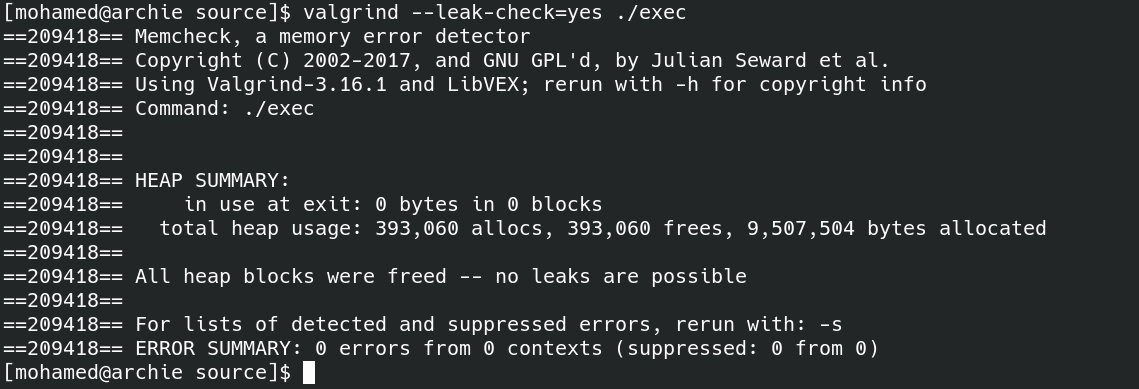
\includegraphics[scale=0.5,width=350pt]{valgrind}
\end{figure}
\end{document}






